\chapter{Introduction}
\label{chap:introduction}

% The function of this chapter (ca. 2 pages) is to introduce the work, place it for the reader in a context. Often a big problem and after some sub-problems needed to resolve the big one. The introduction leads to a problem statement. After state how this work will tackle the (sub)problem and how (“what is done”). The final paragraph can be guide how the thesis is structured. 


%  
%  
% Main feedback, have a clear structure in this chapter, also guide for further work:

% - Introduce and write for a redear, place the work
% - Work towards a problem statement, based on analysis before. Back up assumptions and motivation by literature.
% - At end, state you aims, link to previous analysis and maybe literature. Here can be specific.




% Main point is to write for the reader, from his/her perspective and turn it to your take on the subject. Back-up statements, how the issue developed by references.

% Paragraph 1, intro to X-ray analysis and why it is important.
Properties of materials are strongly related to their nm-scale composition and structure \brynjar{cite? MacArthur?}, where the main tools for studying nanoscale structures is scanning and transmission electron microscopes (SEM and TEM), and the composition can be studied by exciting the material and analyzing the characteristic X-rays emitted \cite{goldstein_scanning_2018,carter2016transmission}.
% In SEM and TEM the excitation of the material is done by the electrons in the electron beam, and the emitted X-rays are analyzed by energy dispersive X-ray spectroscopy (EDS).
There are three main techniques in electron microscopes for analyzing characteristic X-rays: energy dispersive X-ray spectroscopy (EDS), wavelength dispersive spectrometers (WDS) and X-ray fluorescence (XRF) \cite{jenkins_xrayspectroscopy}.
In EDS the electron beam of the microscope excites the material that generates the characteristic X-rays, which are detected and sorted by energy in an accumulating digital histogram, where the energy resolution is limited to around 120 eV, the compositional detection limit is around $\textnormal{C}=200^{-6}$, and the spectrum is affected by different artifacts \cite{goldstein_scanning_2018}.
In WDS the material is excited by electrons as in EDS, but the detector is tuned to only one wavelength at a time, which gives a high energy resolution around 10 eV and a high quality spectrum, i.e. a high peak-to-back-ground ratio and limited number of artifacts, but the WDS technique is less convenient to use and much slower than EDS \brynjar{cite?}.
In XRF the material is excited by a beam of high-energy X-rays or gamma rays, which gives XRF detectors a very low detection limit (around $\textnormal{C}<5^{-6}$ for bulk and $\textnormal{C}<2^{-9}$ for thin samples \cite[Ch. 13.3.5]{xrf_detection_limit}) and the possibility of being handheld, but the photon beam can both penetrate deeper into the material and is not as focused as the electron beam, resulting in a much lower spatial resolution than EDS \cite{xrf_spatial_resolution}.
\ton{Ok to mention that XRF can be handheld, but not EDS? Feels on the edge of relevant.}
% cite ?  https://www.ncbi.nlm.nih.gov/pmc/articles/PMC3681684/
Despite the limited energy resolution and detection limit, as well as a spectrum with artifacts, the EDS technique is  the most used analytical technique in research and industry for electron microscopy \brynjar{cite?}, both for SEM and TEM.








% [Now reader has an intro, and alerted to some weak sides that can be addressed]

% [Could have a schematic figure or a flow diagram. You will addres a) experimental setup characteristics as efficiency, energy resolution, …and data treatment. Terms are introduced that you measure or try to improve on later. Can in later round add extra terms [with reference]. What is done is spelled out later. ]


% Paragraph 2, introduce the experimental setup characteristics and data treatment that can influence the performance of EDS analysis.
In order to improve the performance of SEM EDS, it is necessary to examine the entire process from signal creation to interpretation, including signal analysis.
By doing so, it becomes possible to identify and address any factors that may be responsible for reduced performance.
While the quantum mechanics behind the creation of characteristic X-rays by high-energy (>1 kV) is well understood \cite{hollas_modern_2004,goldstein_scanning_2018}, the signal can be influenced by a range of factors between its creation and detection.
As such, it is important to have a comprehensive understanding of the experimental setup characteristics, the acquisition parameters, and the possible post-acquisition data treatment in order to improve the performance of SEM EDS.
Experimental setup characteristics, such as energy resolution, signal-to-noise ratio \cite{fiori_peak_background_1982}, detector efficiency, partial absorption of the signal, collection angle, working distance, linearity between generation and detection, shadowing, and stability of resolution and peak positions, all play a crucial role in the quality of the acquired data \cite{goldstein_scanning_2018} \ton{Do you want a citation on each parameter?}.
Similarly, acquisition parameters, including beam energy, probe current, process time, dwell time, dead time, and sample type, can also influence the quality of the signal \cite{goldstein_scanning_2018}.
In addition to the experimental setup and the acquisition parameters, post-acquisition data treatment can have a significant impact on the compositional results.
Post-acquisition data treatment can include making method-specific assumptions, model fitting, and noise treatment \brynjar{citation?}.
Although the principles and some hardware used for SEM and TEM EDS are similar, the workflow and final results can differ significantly.
Notably, TEM samples are typically much thinner, at around 100 nm, whereas SEM samples are usually bulk specimens.
Additionally, the beam energy differs, with TEM typically using 100-300 kV, while SEM typically uses 1-30 kV.
The latter energy range is similar to the energy of characteristic X-rays central to this work.
The thin samples used in TEM allow for the absorption effect to be ignored, while the high beam energy allows for the overvoltage effect to be ignored \cite{carter2016transmission}.
These effects and others, must be taken into account in SEM EDS analysis, as the bulk specimens used in SEM can lead to partial absorption of the signal, while the lower beam energy makes the overvoltage effect significant.
The different characteristics which potentially influence the performance of EDS analysis are illustrated in \cref{fig:parameters}.
Characterization of key parameters is necessary to ensure that a spectrum is acquired correctly, and the detector is operating properly, potentially revealing the need for correction.


% figures/intro_parameters.png
\begin{figure}[ht]
    \centering
    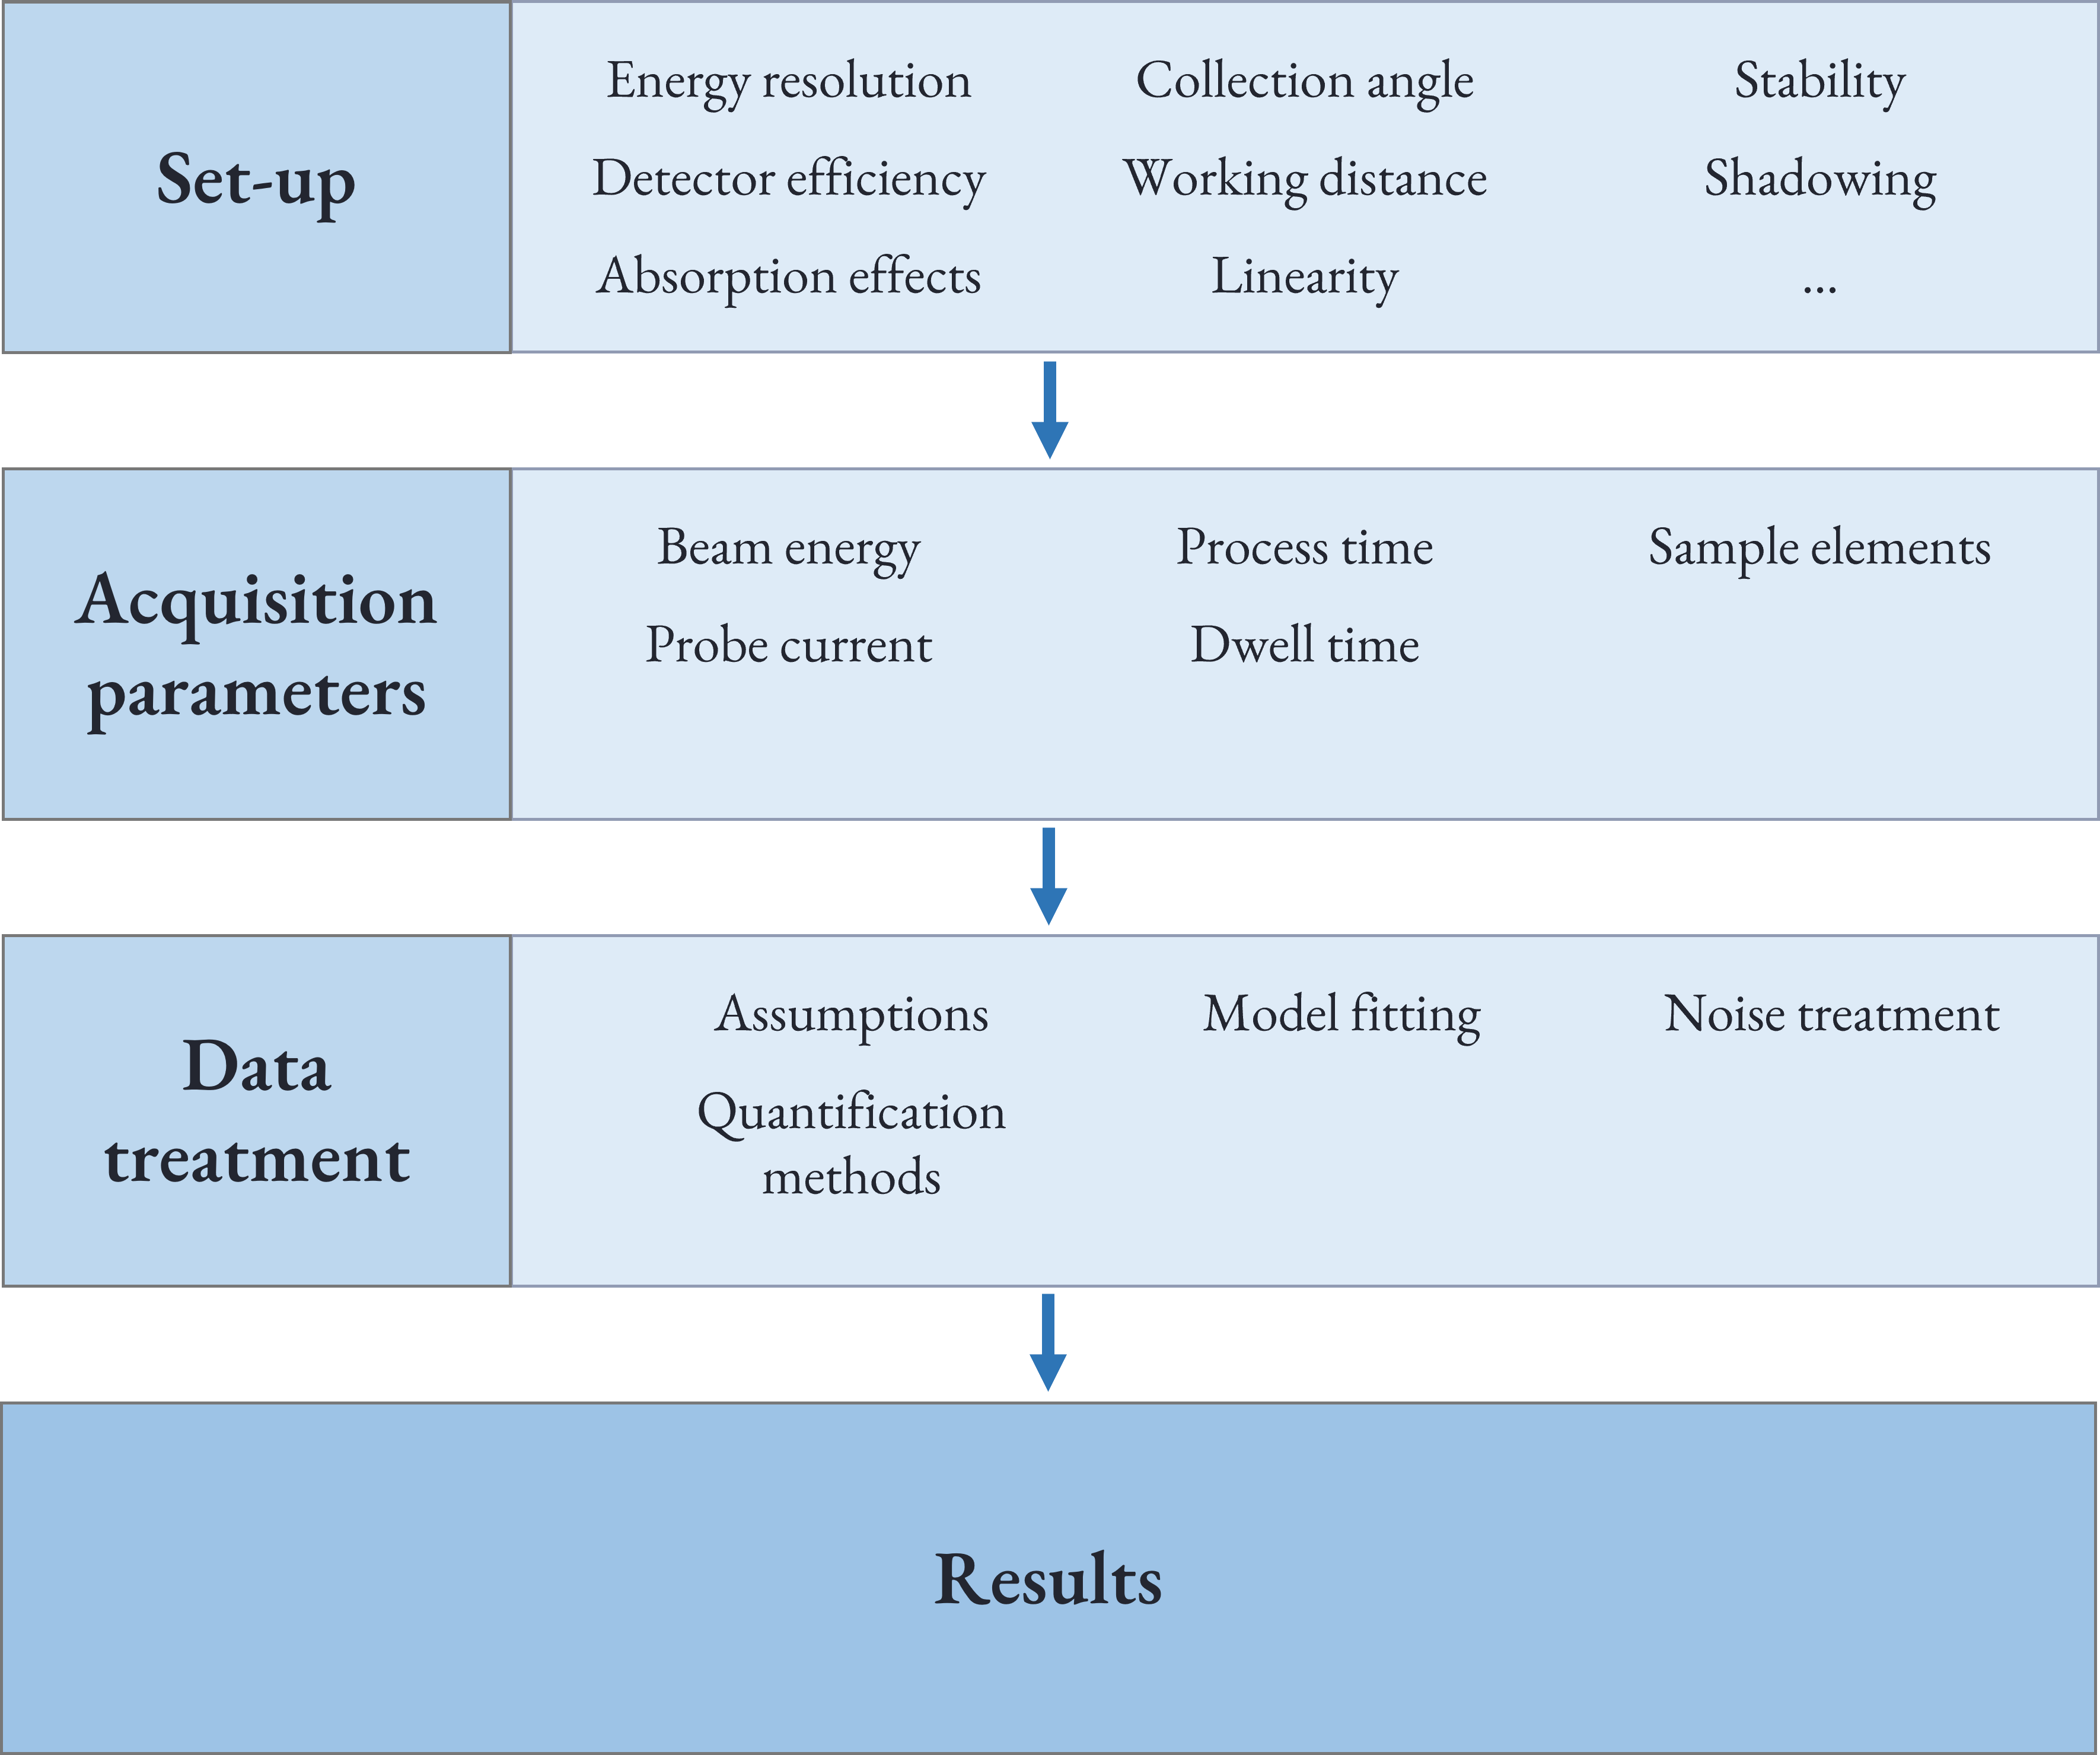
\includegraphics[width=0.8\linewidth]{figures/intro_parameters.png}
    \caption{
        Illustration of parameters that can affect the performance and results of SEM EDS in the three groups.
        This work focuses on some parameters, with the aim of improving the performance of SEM EDS.
        \ton{Is this the type of figure you had in mind?}
    }
    \label{fig:parameters}
\end{figure}






%%%%%% Paragraph 3: open science and open source software
An additional challenge to improving EDS is that the data treatment in commercial software systems is often not transparent and lacks sufficient open documentation.
This can limit the ability to improve compositional analysis for a given setup and data set.
Typically, only default quantification methods, such as Cliff-Lorimer \cite{CL1975}, are included, while alternative methods, such as optimized correction methods that address weaknesses of default quantification routines and factorless quantification \cite{nilsen_factorless_2021}, are not be available.
In recent years, there has been a growing movement towards open science \cite{opensource_2013}, which has led to an increasing role for open-source tools in EDS analysis.
Community-driven freeware and open-source software have gained importance in the EDS community, for example through the development of open file formats such as .msa and .emsa \cite{iso_emsa} and open source software for data analysis.
For SEM EDS analysis, the main non-commercial software is DTSA-II \cite{dtsaii_1_getting_started}, which is developed at NIST by Nicholas W. M. Ritchie, inspired by the original DTSA microanalysis software developed by Chuck Fiori, Carol Swyt-Thomas, and Bob Myklebust.
For TEM EDS analysis, the Python library HyperSpy \cite{hyperspy_1.7.1} is likely the most used open-source software \brynjar{cite?}.
HyperSpy has the advantage of being Python-based, which has become a primary programming language for scientific and collaborative work.
This structure enables EDS analysis to benefit from the integration of algorithms from other fields, such as statistics or machine learning, available in Python libraries such as SciPy \cite{2020SciPy}.
Therefore, HyperSpy is a flexible and dynamic platform available for advancing EDS data analysis.





% [Try here to describe your goals and the work that will be done, based on the intro and analysis what is available, and with limitations, as described before. Think first aim is on track, where the second is more ambitious and might need reformulating. Try to be specific and spell out/back-up by references where you go further]



%%%%%%% Paragraph 4: Python notebook for calibration of SEM EDS
Electron microscopy plays a vital role in materials characterization in both academic and applied research, and there is still room for improvement in the quantitative analysis of EDS data.
To address this, the relevant characteristics of the setup need to be determined.
In the case of TEM EDS, a common approach involves analyzing a spectrum of a thin NiO-film \cite{egerton_nio_characterization_1994,ted_pella_nio_tem_2019}.
Nylund \cite{nylund_evaluation_2017} and Skomedal \cite{skomedal_improving_2022} have developed a Python notebook to extract characteristics, such as offset and energy resolution \brynjar{list all parameters?}, but even though the reports are available through NTNU Open, the notebooks are not publically available to the electron microscopy community.
Moreover, the notebooks are less suited for the low voltages commonly used in SEM, as Nylund and Skomedal worked with TEM and STEM.
Reference values for characteristics like Fiori P/B, \brynjar{parameter 2, and parameter 3 (with citation)} available in the literature, but the values are specified for older Si(Li) type of EDS detectors and may not apply to modern silicon drift detectors (SDDs) \cite{sdd_lechner_2001}.
To fill this gap, a Python notebook that calibrates and does a status check of an EDS setup will be developed and published, including transparent documentation.
The main focus will be SEM EDS, but the notebook will also be applicable to TEM EDS.
Following the notebook will be a proposition for a SEM EDS tailored test specimen.
This work will contribute to improving the EDS setup and acquisition of EDS data, which will aid the quantitative analysis of EDS data, and hence advance the field of materials science.




%%%%%%% Paragraph 5: the more hairy goal of adding bulk quantification to HyperSpy
A second, more ambitious, goal is to develop open-source software for bulk quantification of EDS data, as an addition to the HyperSpy package.
The default approach for bulk is a ratio approach with a sensitivity factor, as for the now implemented Cliff-ratio method that is accepted for thin specimen geometries as used in TEM, but bulk specimen needs an iterative and model-based correction routine for atomic number (Z), absorption (A) and fluorescence (F) \cite{goldstein_scanning_2018}.
These so-called ZAF-corrections are not implemented in HyperSpy and analysis run under the thin-film approximation.
This work aims to explore whether iterative ZAF corrections in the HyperSpy environment, or if an alternative quantification routines such as factorless internal composition determination \cite{nilsen_factorless_2021} \ton{is this correctly phrased?} or other methods could extend EDS analysis within HyperSpy to the low energy range and bulk specimen geometry.





Last paragraph will be a guide how the report is build up, as in the project report. Added later.









